% Author: Dominik Harmim <xharmi00@stud.fit.vutbr.cz>
% Author: Vojtěch Hertl <xhertl04@stud.fit.vutbr.cz>

\documentclass[a4paper, 11pt]{article}


\usepackage[czech]{babel}
\usepackage[utf8]{inputenc}
\usepackage[left=2cm, top=3cm, text={17cm, 24cm}]{geometry}
\usepackage{times}
\usepackage{verbatim}
\usepackage{enumitem}
\usepackage{graphicx} % vkládání obrázků
\usepackage[unicode]{hyperref}
\hypersetup{
	colorlinks = true,
	hypertexnames = false,
	citecolor = red
}


\newcommand{\RNum}[1]{\uppercase\expandafter{\romannumeral #1\relax}} % makro na sázení římských čísel


\begin{document}


	%%%%%%%%%%%%%%%%%%%%%%%%%%%%%%%% Titulní stránka %%%%%%%%%%%%%%%%%%%%%%%%%%%%%%%%
	\begin{titlepage}
		\begin{center}
			
\includegraphics[width=0.77\linewidth]{inc/FIT_logo.pdf} \\

			\vspace{\stretch{0.382}}

			\Huge{Simulační studie} \\
			\LARGE{\textbf{Rozvoz jídla firmou FreshBox}} \\
			\Large{Tým ModelX, varianta 2: Doprava zboží nebo osob}
			\vspace{\stretch{0.618}}
		\end{center}

		\begin{minipage}{0.4 \textwidth}
			{\Large \today}
		\end{minipage}
		\hfill
		\begin{minipage}[r]{0.6 \textwidth}
			\Large
			\begin{tabular}{l l l}
				& \textbf{Dominik Harmim} & \textbf{(xharmi00)} \\
				& Vojtěch Hertl & (xhertl04) \\
			\end{tabular}
		\end{minipage}
	\end{titlepage}



	%%%%%%%%%%%%%%%%%%%%%%%%%%%%%%%% Obsah %%%%%%%%%%%%%%%%%%%%%%%%%%%%%%%%
	\pagenumbering{roman}
	\setcounter{page}{1}
	\tableofcontents
	\clearpage



	%%%%%%%%%%%%%%%%%%%%%%%%%%%%%%%% Úvod %%%%%%%%%%%%%%%%%%%%%%%%%%%%%%%%
	\pagenumbering{arabic}
	\setcounter{page}{1}

	\section{Úvod}

	V této práci je řešen proces sestavování modelu[IMS slide 7] pro rozvoz jídla po Brně firmou FreshBox[TODO] a jeho následná simulace[IMS slide 8]. Díky tomuto modelu a simulačním experimentům[TODO] nad ním je možno pozorovat efektivitu a přínos v různých podmínkách. Smyslem experimentů je zjistit, jak kvalitně navržený je systém[IMS slide 7] a zda by se změnou některého z ovlivňujících faktorů mohl zdokonalit. 


	\subsection{Autoři, zdroje}

	Projekt vypracovali studenti Dominik Harmim a Vojtěch Hertl z VUT v Brně, FIT. 

	K technické části této práce bylo využito zdrojů z předmětu Modelování a simulace. Jako zdroj k faktům sloužila webová stránka firmy FreshBox[TODO] a také vedoucí této firmy, Mgr. Silvie Obadalová (obadalova@freshbox.cz).

	\subsection{Ověření validity}

	Ověřování validity[TODO] probíhalo telefonicky a elektronicky s vedoucí firmy FreshBox, magistrou Obadalovou. Na základě této komunikace byla získána všechna data potřebná k experimentálnímu ověřování validity modelu. Validita byla také ověřena pomocí experimentů a srovnáním s realitou.
	\clearpage


	%%%%%%%%%%%%%%%%%%%%%%%%%%%%%%%% Rozbor tématu a použitých metod/technologií %%%%%%%%%%%%%%%%%%%%%%%%%%%%%%%%
	\section{Rozbor tématu a použitých metod/technologií}

	Všechna použitá fakta jsou zprůměrována ze všech získaných informací. \\

	Zákazníci mají předem objednaná jidla od firmy FreshBox, která tato jídla každý den od 6:30 hod. do 12:30 hod. rozváží zákazníkům po Brně a okolí. Firma FreshBox rozváží jidlo A auty, přičemž jedno auto je schopné naložit maximálně B jídel. Každý den se rozváží průměrně C jídel. Firma má na začátku rozvozu již všechna jídla připravena a v 6:30 se připraví všechna auta, do kterých se naloží maximální počet jídel, který je dán kapacitou auta. Naložení jednoho auta průměrně trvá D minut. Rozvoz všech jídel jednoho auta trvá průměrně E minut. Při tomto rozvozu každé auto urazí průměrně F km. Pro rozvoz se požívají auta značky G. Tato auta mají spotřebu H l/100km banzínu/nafty. Když auto rozveze všechna naložená jídla, vrátí se na pobočku FreshBox, aby se mohla naložit další jídla. Tento proces se opakuje tak dlouho, dokud nejsou rozvezena všechna jídla. Jeden zákazník (právnická nebo fyzická osoba) si samozřejmě může objednat více jídel na jedno místo doručení. Průměrná hodnota objednávky jednoho zákazníka v jeden den činí I Kč.

	\subsection{Použité postupy}

	Pro vytvoření modelu byl použit programovací jazyk C++ za podpory simulační knihovny SIMLIB [citace]. Tyto technologie jsou ideální pro řešení zadaného problému, jelikož poskytují všechna potřebná rozhraní k implementaci modelu. Dále byly použity postupy popsané v prezentaci k předmětu IMS k vytváření Petriho sítě[citace] a samotnému programování za použití knihovny SIMLIB[citace].

	\subsection{Popis původu použitých metod/technologií}

	TODO vyjmenovat všechny technologie a autory u nich, např. Knihovna SIMLIB ve verzi ..., autor Dr. Ing. Petr Peringer.
	-- až nakonec, až budu vědět, co všechno se použilo



	%%%%%%%%%%%%%%%%%%%%%%%%%%%%%%%% Koncepce modelu %%%%%%%%%%%%%%%%%%%%%%%%%%%%%%%%
	\section{Koncepce modelu}

	V této sekci se zpracovává návrh konceptuálního modelu[TODO] nad systémem, který je brán jako systém hromadné obsluhy. Při vytváření je potřeba vybrat ze všech údajů ta podstatná pro model. Jak lze vyčíst z rozboru tématu, důležité je, namodelovat všecho, co souvisí se samotným rozvozem. Díky skutečnosti, že časové údaje jsou průměry zjištěných časů, je zřejmé, že bude dostatečné simulovat průběh jednoho dne, přičemž se samozřejmě může den ode dne nepatrně lišit. Na všechny časové údaje při modelování se tedy použije rovnoměrné rozdělení[TODO] s určitým rozptylem. Aby se model zjednodušil, průměrný počet jídel, který se každý den rozváží, se zaokrouhlí, aby byl dělitelný maximální kapacitou aut. Na validitu to má nepatrný vliv, dá se říci, že zanedbatelný. Dále značka auta, spotřeba paliva a cena nejsou pro model důležitá, tyto informace budou použity při zefektivňování systému. Přesto, že tato situace reálně často nenastává, pro lepší experimentování je přidán druhý koncový stav, který znamená, že směna skončí dříve než jsou rozvezena všechna jídla, tedy nějaká jídla zbydou na skladě. Předpokládá se také, že auto, které započne ještě během pracovní směny svůj cyklus, ho celý dokončí.

	\subsection{Popis konceptuálního modelu}

	Model se skládá z dvou hlavních větví. První značí samotný průběh rozvozu jídel a druhá časovač. Druhá z větví jen určuje, jak dlouho probíhá pracovní směna, to je 6 hodin, a jakmile směna skončí, skončí rozvoz jídel. První větev má dvě vstupní proměnné - počet aut a počet jídel. Auto zde slouží jako obslužná linka, kde pokud je některé volné a připravené na rozvoz a zároveň jsou ještě nějaká jídla na skladě, začnou se nakládat. Pokud je však některé z aut připraveno na rozvoz, ale již byla všechna jídla rozvezena, skončí pracovní směna. Po naložení jídel se auto vydá na cestu a všechna jídla rozveze. Po ukončení této činnosti je auto zase volné a připraveno k použití.

	\subsection{Forma konceptuálního modelu}

	Model je vizualizován pomocí Petriho sítě[TODO] v příloze A.




	%%%%%%%%%%%%%%%%%%%%%%%%%%%%%%%% Architektura simulačního modelu %%%%%%%%%%%%%%%%%%%%%%%%%%%%%%%%
	\section{Architektura simulačního modelu}



	%%%%%%%%%%%%%%%%%%%%%%%%%%%%%%%% Podstata simulačních experimentů a jejich průběh %%%%%%%%%%%%%%%%%%%%%%%%%%%%%%%%
	\section{Podstata simulačních experimentů a jejich průběh}




	%%%%%%%%%%%%%%%%%%%%%%%%%%%%%%%% Shrnutí simulačních experimentů a závěr %%%%%%%%%%%%%%%%%%%%%%%%%%%%%%%%
	\section{Shrnutí simulačních experimentů a závěr}



	%%%%%%%%%%%%%%%%%%%%%%%%%%%%%%%% Citace %%%%%%%%%%%%%%%%%%%%%%%%%%%%%%%%
	\clearpage
	\bibliographystyle{czechiso}
	\renewcommand{\refname}{Literatura}
	\bibliography{dokumentace}



	%%%%%%%%%%%%%%%%%%%%%%%%%%%%%%%% Přílohy %%%%%%%%%%%%%%%%%%%%%%%%%%%%%%%%
	\clearpage
	\appendix

	\section{Petriho síť}
	\begin{figure}[!ht]
		\centering
		\vspace{-1.2cm}
		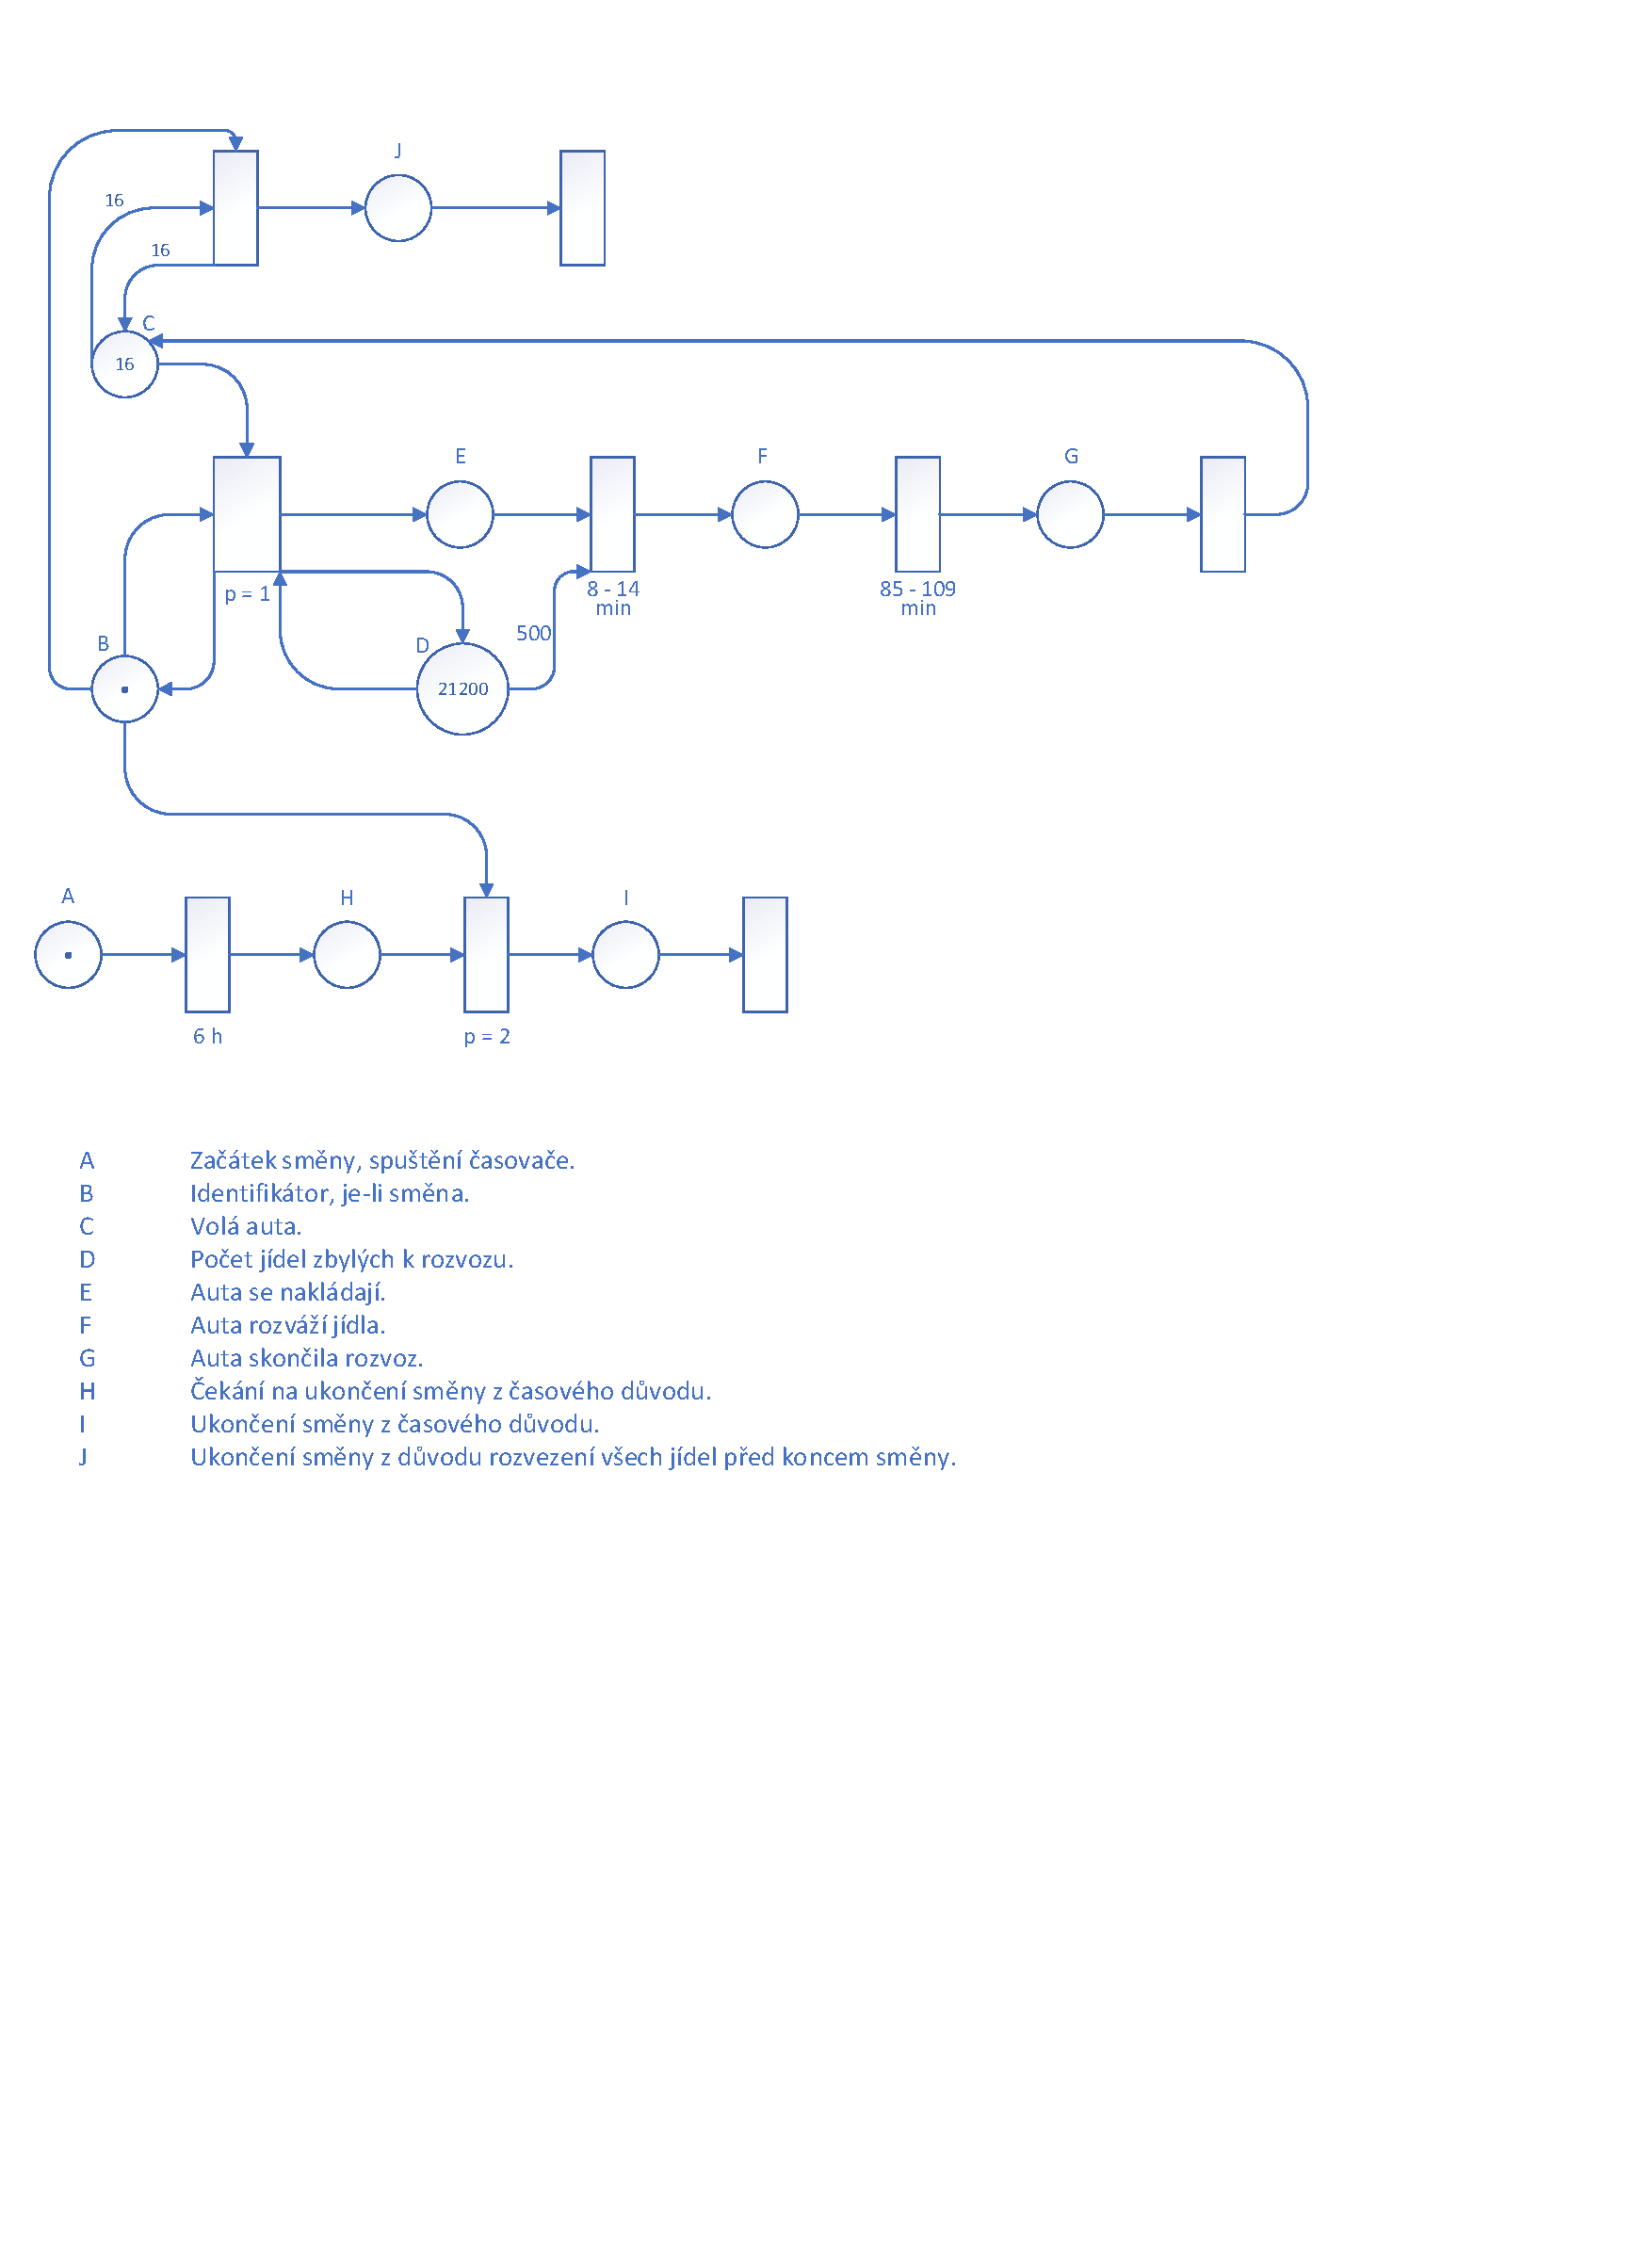
\includegraphics[width=0.95\linewidth]{inc/petri_net.pdf}
		\caption{Petriho síť}
		\label{figure:petri_net}
	\end{figure}



\end{document}